\begin{figure*}[t]
\begin{minipage}[t]{3.5in}
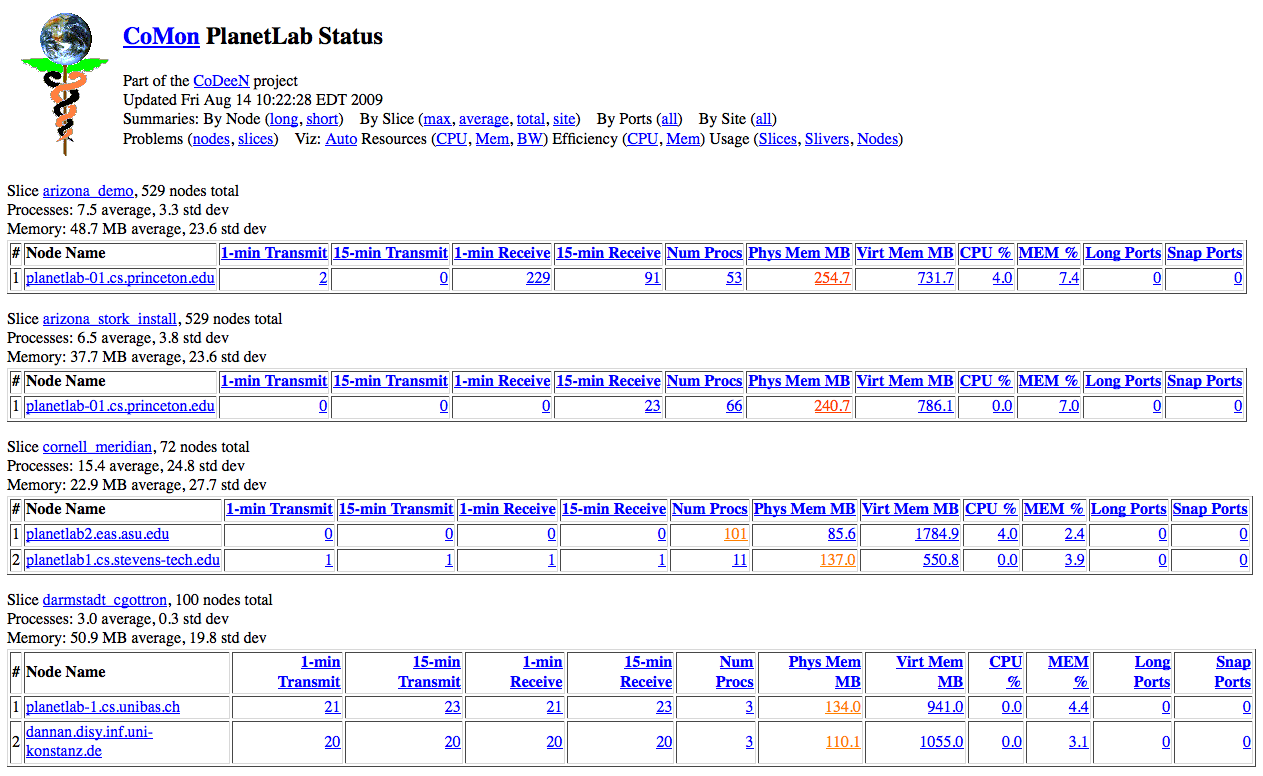
\psfig{file=pic_sliceprob.ps,width=3.5in}
\caption{Anomalous VM instances reported per application. Note that
these applications have between 72-529 VM instances, and 1 or 2 instances
per application are being flagged due to anomalous numbers of processes
or physical memory consumption.}
\label{fig_comon_anomaly}
\end{minipage}
\hspace{.25in}
\begin{minipage}[t]{2.75in}
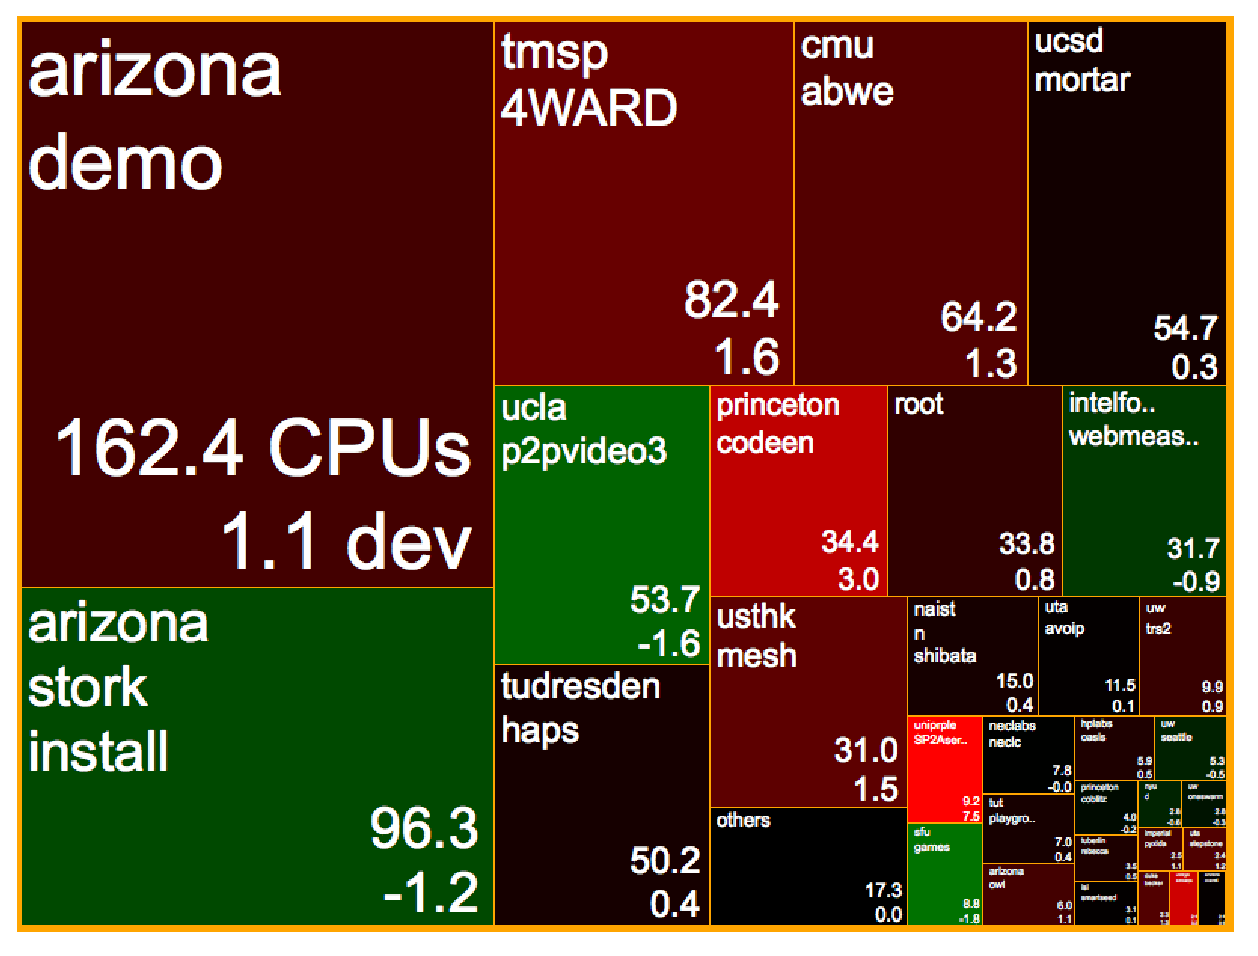
\psfig{file=pic_treemap.ps,width=2.75in}
\caption{Treemap of resource consumption on PlanetLab. Rectangle size
is proportional to CPU consumption, while color indicates deviation
from weekly average. Red indicates higher than average, while green
indicates lower than average.}
\label{fig_comon_treemap}
\end{minipage}
\end{figure*}

\subsection{The CoMon Monitoring and Visualization Framework}
\label{sec:comon}


The CoMon monitoring system is a general-purpose scalable monitoring
system that was originally developed to support the PlanetLab global
network testbed and the applications that use it~\cite{CoMon}. We run
it as a hosted service, and it currently supports not only PlanetLab,
but also one dozen other projects, ranging from other testbeds to a
variety of applications. For PlanetLab alone, the system is collecting
over 350 thousand data points every five minutes, all of which are
inserted into its custom database, and which can be queried
individually, displayed in tables, or presented as graphs. While these
numbers may not be particularly large in and of themselves, all of this
is accomplished using a dual-core commodity server with only 4
Gigabytes of memory and a single 14-disk shelf in a RAID6
configuration. In comparison, published reports for the world's
largest MRTG system indicate that its hardware usage is 8 processors,
16GB of memory, and 32 disks in a RAID-10 configuration~\cite{Plonka}.

% Application Buffer-Cache Management for Performance: Running the World's Largest MRTG
% David Plonka, Archit Gupta, and Dale Carder - University of Wisconsin-Madison

%Pp. 63-78 of the Proceedings of the 21st Large Installation System Administration Conference (LISA '07)
%(Dallas, TX: USENIX Association, November 11-16, 2007). 

What differentiates CoMon from many of the other monitoring systems in
use is that is has no permanent database configured for most of the
data it collects. Other than data collection, virtually all data
processing is performed lazily, only as needed when queries are made
to the data. In database systems, eager processing is viewed as a way
of performing some possibly unnecessary processing in order to reduce
the latency of any future requests. In CoMon, lazy processing allows
most processing to be deferred, and often not performed at all, since
most data in the system typically requires no long-term processing.
When data is requested, CoMon uses its intelligent disk layout to
reduce the number of seeks involved in fetching content, and as a
result, typically keeps query time, even for historical data, to well
under one second.

CoMon already has demonstrated its utility across a range of
applications due to its origins on the PlanetLab testbed. In
particular, one of the uses of CoMon is monitoring resource
consumption for all virtual machine (VM) instances in PlanetLab. For
privacy reasons, PlanetLab exports aggregate consumption of resources
on a virtual machine basis, rather than exposing the processes within
each VM. CoMon typically records usage for 25-30K simultaneous VM
instances across the nearly 1000 nodes in PlanetLab. Any Planetlab
experiment can run across any number of nodes, and CoMon performs
anomaly detection across the VM instances of each experiment. As a
result, application authors are alerted to which instances of their
applications appear different from the other instances, solely based
on resource consumption. An example of this kind of reporting is shown
in Figure~\ref{fig_comon_anomaly}. Here, only the anomalous VM
instances of each application are being highlighted, with summary
information provided for all of the conforming instances. This data
reduction allows developers to quickly examine the reported anomalies
and determine whether to act on them. A number of application
developers have used this information to start the debugging process
on their distributed systems. We believe that by extending CoMon to
operate on messages between application processes, the level of detail
generated will provide even more utility to application developers.

For this context, the larger advantage of lazy processing with no
database is that no on-disk structures need to be allocated in
advance, so if a new set of data items is introduced, they are stored
to disk just as all other data is stored. By removing the need to have
structured storage in place before receiving data, CoMon can eliminate
the overhead of preparing tables for insertion. Likewise, if the
format of data items changes over time, no reformat of any database is
necessary since the new item format can coexist with older formats. By
making CoMon store its parsing information along with the data, CoMon
can automatically handle different data versions for the same data
field.

The research we need to perform for CoMon is how to make it seamlessly
interoperate with PADS, especially for automatically-inferred data. We
believe that the existing infrastructure is sufficiently scalable,
based on our PlanetLab experience. However, all configuration in CoMon
is currently performed manually, and the process of having all CoMon
configuration be performed automatically has not been
considered. Furthermore, since CoMon will be the prime visualization
and analytics system, we need to determine what kinds of analytics and
visualization is appropriate for previously-ignored application data.
An example of visualization for PlanetLab is shown in
Figure~\ref{fig_comon_treemap}, where behavior of all applications
running across PlanetLab is shown in one image. For each application,
resource usage across all VMs is aggregated, and each is represented
as one box in a treemap~\cite{x} format. The size of each box
represents the resource consumption, and the color represents the
number of standard deviations from its weekly average. Using this kind
of visualization, operators can see which applications are behaving
unexpectedly, how severe their behavior is, and how much of an impact
it is having on the overall testbed. By visualizing this data,
PlanetLab operators can quickly determine where to spend their time to
achieve the most benefit.  At a first step, we intend to explore how
to perform this kind of visualization for a range of applications with
as little operator configuration as possible.  Given our experience on
PlanetLab with solely resource consumption, we believe that many
problems can be identified with relatively little information. To
extend this kind of work, we are likely to examine correlation of data
from multiple data sources, which we have not performed in this
context.  Given our experience with anomaly detection for PlanetLab
experiments, we believe that correlation of multiple data sources may
provide similar insights.
